
\setlength\parindent{0cm}

\subsection{Introduction}
We will now review a number of literary sources which fall within the context of path-finding methods and procedural content generation to explain how these techniques work and to establish how these may be used within the project to either help implementation or optimisation of the project in it's latter stages.  


\subsection{Background and inspiration}
The inspiration for this project was based around pushing performance and analysing both level generation and path-finding approaches to find a common area where these methods can be combined to improve run-time performance and to allow testing of the quality of both the terrain and path that is built in terms of complexity against the amount of nodes required to build a logical path and any deviations that are made to the path due to constraints posed by the terrain. 

For a time line of various path-finding techniques please refer to figure \ref{timeline}

\subsection{The history of computer graphics}
As mentioned  
\subsection{Procedural Level generation Techniques}
There are a variety of ways to generate either 2d or 3d geometry within a program this section will discuss the documented methods and compare them in terms of usability and performance.

The paper \cite{LG-Survey} examines the different layers of a game that can be procedurally generated this includes a section on game space for levels or maps and defines these both abstract or concrete methods for generation of both indoor and outdoor environments as well the paper gives a taxonomy of commonly used procedural content generation techniques.  

\subsubsection{The Diamond-Square algorithm}
This method of level generation was proposed by \cite{DSA2} is based off fractal subdivision to generate randomised terrain based on two steps which are split into the diamond step  and the square step hence the algorithms name.\\\\ The diamond step of this algorithm uses the edge points of a square to generate a random value in the midpoint then the square step of this algorithm performs the same function however uses the edge points of the diamond made previously which gives a square as the result. \\\\The algorithm is recursive meaning that it performs multiple passes through each step with the generated surface gaining detail every pass however the increase is due to more geometry being created each pass this means the algorithm can be memory intensive due to the size of array used to store the height values being a power of two + 1 this means for eight passes through the algorithm the array would need up to 256KB memory if storing floating point values \cite{LevelDSA}.

\subsubsection{The marching cubes algorithm}
The marching cubes algorithm is another method that can be used to generate terrain it was first proposed in 1987 by \cite{marching} the algorithm was used to output three dimensional images from medical scan results and does this by creating polygons from the density of surfaces contained within a three dimensional array.\\\\The algorithm works by first taking in a user defined start point within a cube in three dimensional space and starting to create triangles then using intersection testing against the cube to determine where the generated triangles end then we move or march to the next point within the cube an example of this from the paper \cite{marching} is shown below and shows how the 3D space and cube are set up.     

\begin{figure}[ht!]
	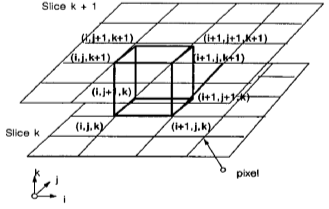
\includegraphics[width=0.5\textwidth]{images/Marchingcubes}
	\caption{The 3D space of a marching cube}	 \label{cube}
\end{figure}

\subsubsection{Height-map generation and Rendering}
A height map is a grey scale image that makes use of depth to create a section of terrain with areas where the terrain to be raised being shown as brighter and lower areas shown as dark for most height maps digital noise is used to produce a suitable terrain for an example of the output that is produced by a height map please refer to figure \ref{noise} the algorithm for creating digital noise will be detailed below. 

\subsubsection{Perlin Noise}
\label{Perlin}
To create the image \ref{noise} Perlin Noise was used this is a gradient based noise developed by Ken Perlin in 1983 \cite{perlin} to create procedural textures using the algorithm outlined below. 
\begin{itemize}
\item Get an input point of the image 
\item Loop through the neighbours of this point
\item Generate a pseudo-random gradient vector.
\begin{figure}[h]
\centering
\item perform the following calculation
\begin{equation}
\label{eq:Noise}
G \cdot(P-Q)
\end{equation}
\caption{G= gradient vector P = input point Q = Neighbouring point}
\label{noise:eq}
\end{figure}

This equation will give the value of P where G is equal to 0 at point Q.
\item Finally you Interpolate between the the points down to your point, using an S-shaped cross-fade curve e.g( 
\begin{math}(eg: 3t^2-2t^3)\end{math}) this will give the weighting applied in each dimension.This step will require computing of the curve n times, followed by 2n-1 linear interpolations to get the final result.
\end{itemize}

\subsection{Path-finding Techniques}
This section will analyse some of the key path finding techniques that would address the problem posed within the project including an analysis of past work done in this area will be given with the aim to analyse how this can be utilised and expanded within the project. 
\subsubsection{Dijkstra's algorithm}
The algorithm for path finding presented by Edsger Dijkstra in 1959 \cite{dijkstra} allows searching of a weighted graph to determine the shortest route through a set of nodes by working out the shortest path from one node to every other connected node in the graph with only the shortest distance being chosen from one node to the next this technique is known as a uniform cost search. The nodes can be used to represent space within either a two dimensional grid or a point in three dimensions.\\\\ This method can be used within the project as the cost of travelling between nodes can be calculated as the euclidean distance between the nodes this will allow us to remain with vector calculations which would benefit a GPU based implementation. If we look at figure \ref{timeline} it is shown there have been a number of developments to this method of path-finding the main adjustments that are beneficial to the project will be discussed below.
\paragraph{Algorithm details}
Dijkstra's algorithm uses the following steps to calculate the shortest path from a starting node to any other node.

\begin{enumerate}
	\item Set up graph of nodes with all distances being infinite except the starting node which is initialised at zero.
	\item Make sure all distances are set temporarily with the starting node being set permanently
	\item Find the neighbours of active node and from there calculate their distance to the starting node using the weights on the edges which are determined by distance.
	\item The neighbouring node with the lowest distance is chosen to become the next node from the start we then update the distance at the starting node and set the next node to active.
	\item set the chosen nodes distance to permanent and repeat steps three and four until there are no neighbouring nodes in the graph with temporary distances.      
\end{enumerate}
 
\paragraph{Developments to graph based path finding}
There have been a multitude of developments to graph based path finding techniques these include some of the key methods mentioned in \ref{timeline}  the ideology of these techniques and their benefits in the context of this project will be discussed.

The first development to graph based techniques that is interesting is the article by \cite{goodchild} this was where the traditional orthogonal approach to building paths was modified due to the fact that errors were produced with straight line and smoothly curved paths the solution was to look at using both the orthogonal and diagonal steps to reduce the errors produced such as deviation from the path and this also prevents the path from becoming too long.

Another development of interest is the creation of a spread based algorithm for path-finding that was first proposed by \cite{califano} the origin of the splash (structural pattern localization analysis by sequential histograms) algorithm was to identify patterns in amino acids and other uses within the field of computational biology relying on sparse pattern matching techniques.\\\\  The splash is shown in \cite{califano} to be both memory and computationally efficient when compared with other path finding methods due to the utilisation of sparse pattern matching this is of value as it allows for faster processing of a path that contains pattern and using the splash algorithm could be beneficial due to the parallelizable nature of that this algorithm uses to search through data.    


\subsubsection{Path finding in games}
\label{pfg}
Path finding is an area of artificial intelligence widely used in games to allow computer controlled characters to walk on the geometry that makes up a game world or level the paper by \cite{pathfinding-games} describes the method for path finding on geometry by first building a navigational mesh which describes the parts of a given world or level can be traversed or using a node based waypoint system which is traditionally based on the visibility of one node to the next which allows for traversal of the geometry.\\\\ There is also a breakdown of path finding techniques into directed and undirected methods with directed methods such as the A* algorithm which combines the cost based searching of nodes or a navigational mesh with a heuristic search to a goal this allows for greater efficiency over Dijkstra's algorithm which is a important consideration for many games.

\subsubsection{The A* algorithm}
The A* or A star path-finding algorithm was first proposed in 1968 the paper \cite{A*} this method for path-finding uses a heuristic based search to find the shortest route for a given weighted graph to a goal node or set of goals.\\\\ There are many benefits to using this algorithm these include storing previously any visited nodes that do not lead to the goal this helps to prevent backtracking and eliminate infeasible solutions leading to a reduction in the search space thus an increase in runtime performance although this comes with an increased memory overhead as a result of using two lists over one list to store the path.   
\subsubsection{Analysing the quality of path-finding techniques}
\label{quality}
The niche of this project is that there has been no previous attempt to quantify the quality of procedural level development techniques with regards to ease of path-finding as a factor for the assessment of quality and  to assess the performance of path-finding techniques with regards to the complexity of a terrain that is generated.\\\\ A solution that may be used is to create an artificial intelligence system that can learn from examples and possibly create it's own which will then be assessed to expand on learning to improve response times and fine tune the metric that will be established.\\\\ There are many systems that utilise this method of learning an example of such being the system developed by Google\textsuperscript(tm) in their deep mind department called Alphago which was used to beat the current champion of the game GO\cite{AI-learning}.\\\\ This victory was made possible by training the system with moves made by experts then allowing it to learn from playing against itself the system used two neural networks one to determine promising moves and the other searches ahead of the chosen moves found this reduces the search space allowing this processing to take place.\\\\ A brute force approach would fail due to the magnitude of moves possible in this project the AI system could be utilised to fine tune the metric for level complexity by learning how to score an environment and gradually increasing the consistency of results gathered.

\subsubsection{Previous honours projects}
There has been a previous honours project based on performance of GPU based path-finding. The thesis that was authored by \cite{honours} contains work on a variety of path-finding techniques including Dijkstra, A* and diffusion methods with both a sequential and parallelised implementation the optimised versions of these path-finding approaches which may be utilised in cases of performance bottleneck as this project will not be specifically related to performance but rather the production of an elegant constrained path with a given terrain then scoring this against any path finding technique based on a performance evaluation using the metric that will be established.


There was also a project that proposed a metric for picking good procedurally generated terrain this project looked at the creation of procedural terrain through the use of a height-map and considered what methods can be used for evaluating the quality of a given 3D terrain with descriptions on the implementation of these techniques.\\\\The methods talked about within the thesis \cite{honours2} for quality evaluation of 3D terrain include through the analysis of accessibility this is done by taking the average of a slope in the terrain along with the standard deviation this is then divided by the average slope.\\\\This calculation if higher than one represents a better terrain than if the result is lower what this does is determine how much of the terrain is accessible by assessing the steepness of slopes on a terrain.\\\\For the project \cite{honours2} it was said that a point is accessible for a building if the slope is less than twenty six degrees or where the dot product of these points is greater than 0.9 whereas traversable terrain is defined with a dot product result of 0.7  

\subsection{Optimisation techniques}
To optimise the project a wide range of factors and approaches are being considered the purpose and uses of these will be briefly discussed below along with a discussion on how these methods could benefit this project.\\

\subsubsection{Parallelism and parallel programming approaches}
The first approach to address is that of how to get the most performance out of the development platform (PC) one of the main ways to optimise for this platform is the use of parallel programming this will be implemented through the OpenMP API \cite{Openmp}which is built into Visual Studio this will allow for multi-threading of any code running on the central processing unit (CPU) through the use of pre-processor directives to specify sections of code to incorporate parallelism this approach should give a performance increase by utilising the multiple cores in the central processing unit over a sequential implementation that uses a single core.

Other parallel frameworks have been considered however are not at this point set to be implemented these are the MPI (Message Passing Interface)\cite{mpi} which allows for distributed parallelism over a network this would be extremely beneficial to performance as the host PC which is executing the program would have more resources available however this approach can have issues mainly due to the communication being network based meaning that bandwidth can affect the performance of a program to produce a performance decrease due to the time taken to communicate over the network it is unlikely that the project will utilise this technique however when testing this may be useful for running multiple instances of the project with different parameters. 

\subsubsection{Graphics Processing Unit (GPGPU)}
GPGPU(General Purpose Graphics Processing Unit) programming allows the user to run non graphics based code on the GPU this is beneficial due to the amount of processing cores that the GPU contains over the central processing unit allowing dramatic performance increase however there are a number of drawbacks to this approach and it can only be used within certain problem area's.\\\\ GPGPU programming is a good fit to math based problems over large data sets in comparison to problems that branch through sections of code this is due to the way data is processed on the GPU this is done by streaming data through the GPU cores in groups known as either wavefronts or wraps which are groups of threads within the GPU and the terminology for these differs depending on the technology used instead of the normal fetch execution cycle of the CPU where instructions and resources are fetched from memory before they are executed or loaded.\\\\ To utilise the GPU for processing we must send the data from the processor to the GPU then perform our operations and finally transfer the answer back to the CPU this is one of the main drawbacks to GPGPU programming as the performance is determined not only by the hardware but also by the speed of data transfer between the CPU and GPU also the size that this data takes up in memory will impact on the time taken to transfer from one to the other.\\    

The use of GPGPU techniques for parallel programming were only recently applied to AI because of the branching nature of the problems in this area it has always been considered that  the AI system discussed in \ref{quality} used a distributed system to utilise the hardware resources of multiple machines to carry out consecutive parts of the processing which is passed back to a host machine this is what allowed the massive amount of processing power required by the alphago system to process the best moves at every point of a match. 

\subsection{Commercial packages}
There exist a number of commercial applications that fall within the context of this project most of these are contained within  games engines which contain ways to generate levels and to build paths.\\\\ There are also a variety of evolutionary systems which can be used to find the best solution these can be found within lots of packages one example that is notable being journey planning software such as that contained within Google Maps this uses traffic information along with travel method and location to give you the fastest route to a given destination. 

\subsection{Conclusions Drawn}
To conclude in this section we have looked at various methods to implement both path-finding and procedural level generation we also discuss how these techniques can be measured individually and look at methods such as multi-threading and GPGPU programming for optimisation of these techniques.\\\\We have also looked at previous project based within the context of both level generation and path-finding with the final section analysing commercial packages which implement techniques that may be of interest to the project.  
\pagebreak

